\documentclass[oneside, twocolumn, 9pt, english]{extbook}
\usepackage{supertabular}

\usepackage{../../HPpack}
\usepackage{float}

\begin{document}

\begin{titlepage}

    \centering
    \vfill
    {\bfseries
        {\HP \fontsize{40}{35}\selectfont A Guide to Hogsmeade Village}
    }    
    \vfill
    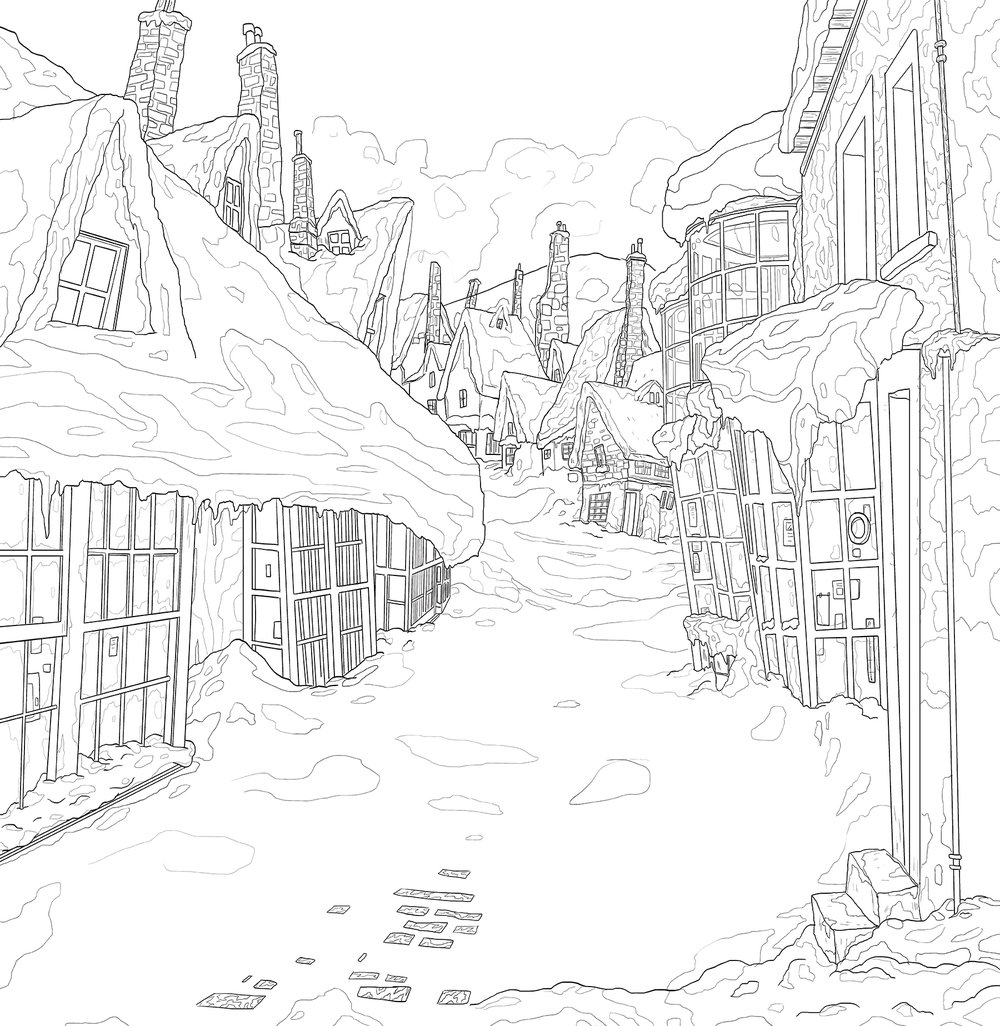
\includegraphics[scale = 0.3]{../../Images/Hogsmeade} % also works with logo.pdf
    \vfill
    {\HP \fontsize{30}{24} \selectfont  Harry Potter \\\&\\ The Role Playing Game}
    \normalsize
    \vfill
    {\HP \fontsize{22}{0} \selectfont Version 1.0 \hfill Jack Fraser}
\end{titlepage}



	\renewcommand\arraystretch{1.5}
\newcommand\basicPerson[2]
{
	\textbf{\textit{#1}}
	
	#2

}

\newcommand\shop[7]
{
	\subsection{#1 (\it #4)}
	
	\begin{supertabular}{@{} r p{6.5  cm} @{}}
		\bf Location:	&	#2
		\\
		\bf Exterior: &		#5
		\\
		\bf Interior:	&	#6
		\\
		\bf Proprietor:	&	#3
		\\
		\bf Inventory:	&	\parbox[t]{6.5cm}{#7}
		\\
	\end{supertabular}
	~
	\\
}

\setlength\parindent{3pt}
%%ShopBegin
\shop{Ceridwen\apos{}s Cauldrons}{Hogsmeade}{\basicPerson{}{} }{}{}{}{}

\shop{Dervish \& Banges}{Hogsmeade}{\basicPerson{a}{a} }{a}{a}{a}{aA full inventory for this shop can be found at the end  of the document}

\shop{Dogweed \& Deathcap}{Hogsmeade}{\basicPerson{}{} }{}{}{}{}

\shop{Dominic Maestro\apos{}s Music Shop}{Hogsmeade}{\basicPerson{}{} }{}{}{}{}

\shop{Gladrags Wizardwear}{Hogsmeade}{\basicPerson{}{} }{}{}{}{}

\shop{Hog\apos{}s Head Inn}{Hogsmeade}{\basicPerson{}{} }{}{}{}{}

\shop{Hogsmeade Station}{Hogsmeade}{\basicPerson{}{} }{}{}{}{}

\shop{Honeydukes}{Hogsmeade}{\basicPerson{}{} }{}{}{}{}

\shop{J. Pippins Potions}{Hogsmeade}{\basicPerson{}{} }{}{}{}{}

\shop{Post Office}{Hogsmeade}{\basicPerson{}{} }{}{}{}{}

\shop{Scrivenshaft\apos{}s Quill Shop}{Hogsmeade}{\basicPerson{}{} }{}{}{}{}

\shop{Shrieking Shack}{Hogsmeade}{\basicPerson{}{} }{}{}{}{}

\shop{Spintwitches Sporting Needs}{Hogsmeade}{\basicPerson{}{} }{}{}{}{}

\shop{The Magic Neep}{Hogsmeade}{\basicPerson{}{} }{}{}{}{}

\shop{Three Broomsticks}{Hogsmeade}{\basicPerson{}{} }{}{}{}{}

\shop{Tomes and Scrolls}{Hogsmeade}{\basicPerson{}{} }{}{}{}{}

\shop{Zonko\apos{}s}{Hogsmeade}{\basicPerson{}{} }{}{}{}{}

\section{Expanded Inventory} \footnotesize 


\expand{Dervish \& Banges}{\invent{Lighting the Spark: An Introduction to Elemental Magic~($\times$3)}{Book of Beginner Elemental spells}{\sickle{10}}
\invent{The Standard Book of Spells~($\times$3)}{Book of Beginner Kinesis spells}{\sickle{10}}
\invent{Reading People\comma{} Reading Minds~($\times$3)}{Book of Beginner Telepathy spells}{\sickle{10}}
\invent{The Dream Oracle~($\times$3)}{Book of Beginner Temporal spells}{\sickle{10}}
\invent{Easy Spells to Fool Muggles~($\times$3)}{Book of Beginner Bewitchment spells}{\sickle{10}}
\invent{Cool Cantrips to Make You Crazy~($\times$3)}{Book of Beginner Psionics spells}{\sickle{10}}
\invent{A Compendium of Common Curses~($\times$3)}{Book of Beginner Curse spells}{\sickle{10}}
\invent{Basic Hexes for the Busy \& Vexed~($\times$3)}{Book of Beginner Hex spells}{\sickle{10}}
\invent{Cures\comma{} Cantrips and Coughs~($\times$3)}{Book of Beginner Healing spells}{\sickle{10}}
\invent{Self\minus{}Defensive Spellwork~($\times$3)}{Book of Beginner Warding spells}{\sickle{10}}
\invent{A Beginner\apos{}s Guide to Transfiguration~($\times$3)}{Book of Beginner Alteration spells}{\sickle{10}}
\invent{The Illusion of {\it Thin Air}~($\times$3)}{Book of Beginner Conjuration spells}{\sickle{10}}
\invent{Further Elemental Studies~($\times$2)}{Book of Novice Elemental spells}{\galleon{1}}
\invent{Achievements in Charming~($\times$2)}{Book of Novice Kinesis spells}{\galleon{1}}
\invent{Detection is the Best Defense~($\times$2)}{Book of Novice Telepathy spells}{\galleon{1}}
\invent{The Future is an Open Book (And so is This)~($\times$2)}{Book of Novice Temporal spells}{\galleon{1}}
\invent{Jiggery Pockery \& Hocus Pocus~($\times$2)}{Book of Novice Bewitchment spells}{\galleon{1}}
\invent{Your Mind\comma{} the Weapon~($\times$2)}{Book of Novice Psionics spells}{\galleon{1}}
\invent{Curses \& Counter Curses~($\times$2)}{Book of Novice Curse spells}{\galleon{1}}
\invent{Hexes to Make Your Head Spin (Literally)~($\times$2)}{Book of Novice Hex spells}{\galleon{1}}
\invent{Magic to Make Others Better~($\times$2)}{Book of Novice Healing spells}{\galleon{1}}
\invent{How Not to be Killed: A Guide for the Discerning Wizard~($\times$2)}{Book of Novice Warding spells}{\galleon{1}}
\invent{Transmutation and Transformative Tricks~($\times$2)}{Book of Novice Alteration spells}{\galleon{1}}
\invent{Making and Unmaking: The Art of Conjuration~($\times$2)}{Book of Novice Conjuration spells}{\galleon{1}}
\invent{Runic Scroll~($\times$4)}{Provides 1 additional rune}{\sickle{8}}
\invent{Small Maps~($\times$5)}{Provides information about a single village or town}{\sickle{5}}
\invent{Large Maps~($\times$5)}{Maps of large cities\comma{} and even entire countries.}{\sickle{8}}
\invent{Fantastic Beasts and Where to Find Them~($\times$3)}{Provides basic information about common beasts}{\sickle{12}}
\invent{The Unlife \& How to Avoid Them~($\times$1)}{Provides basic information about undead \& unliving creatures}{\galleon{1}}
\invent{Monster Book of Monsters~($\times$2)}{A sentient book which viciously attacks people \minus{} inside it has detailed information about common beasts.}{\galleon{1}}
\invent{Rare and Dangerous Magical Creatures Aruond the World~($\times$1)}{Provides basic information about some of the rarer magical creatures found in the world.}{\galleon{2}}
\invent{One Thousand Magical Herbs \& Fungi~($\times$5)}{Contains information about ingredients \& gives hints as to potions they can be used in.}{\sickle{10}}
\invent{Wizarding Biographies~($\times$5)}{Biographies of some famous wizards}{\sickle{7}}
\invent{Potion books~($\times$5)}{Each contains 1d8 random recipes for potions}{\sickle{10}}
}

%%ShopEnd

\end{document}